\clearpage
\SourceLeaf{380}%
\begin{center}\large\bfseries [FLÄCHENTREUE ABBILDUNG EINER EBENE\\ AUF EINE ANDERE EBENE.]\end{center}

Aufgabe. Die Punkte in der Ebene so in eine zweite Ebene zu übertragen, dass jeder unendlich kleinen Figur in der einen Ebene eine von gleichem Inhalt in der andern entspreche.

Es seien die Coordinaten in der einen Ebene $x$ und $y$,\\
\hspace*{1.6em}die correspondirenden in der andern $\xi$ und $\eta$.

\noindent Die \textls[120]{allgemeine} Auflösung ist dann folgende.

Es sei $u$ eine willkürliche Function von $x$ und $\xi$; man mache
\[
y=\frac{\partial u}{\partial x},\qquad \eta=-\frac{\partial u}{\partial\xi}.
\]

\indent Diese Auflösung ist vollkommen richtig und allgemein, und lässt sich leicht geometrisch versinnlichen.

$u$ bedeutet nemlich den hier gezeichneten Flächenraum:
\begin{center}\resizebox{7.2cm}{!}{%
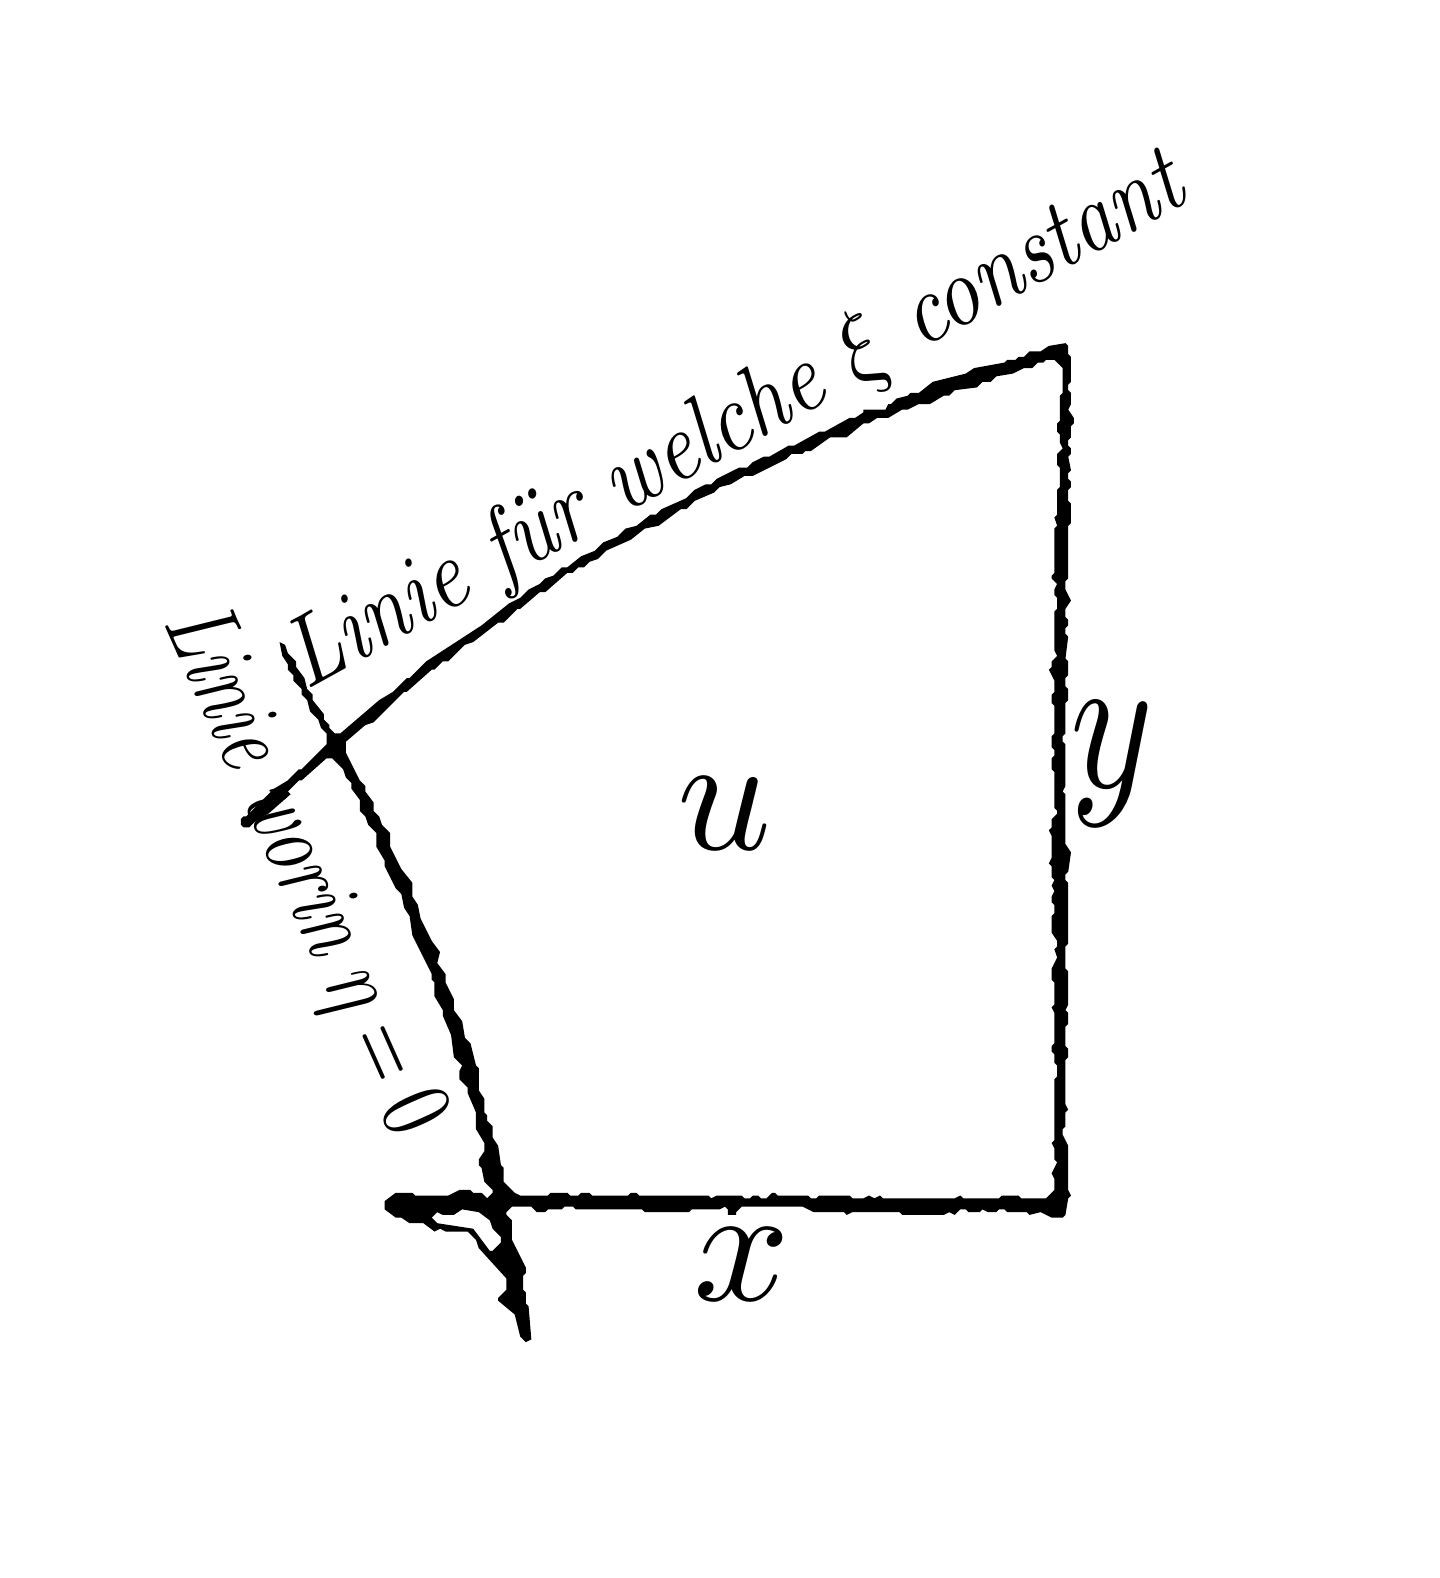
\begin{tikzpicture}[x=1pt,y=-1pt]
\path[use as bounding box] (0,0) rectangle (500,550);
\path[fill=black,draw=none,even odd rule]
(375,114) -- (369,115) -- (366,117) -- (362,117) -- (360,119) -- (358,119) -- (357,120) -- (354,120) -- (353,121) -- (342,123) -- (339,125) -- (327,128) -- (322,132) -- (319,132) -- (318,133) -- (314,134) -- (312,136) -- (311,136) -- (310,138) -- (302,138) -- (302,139) -- (299,141) -- (297,141) -- (288,146) -- (286,146) -- (277,151) -- (275,151) -- (268,155) -- (266,155) -- (262,157) -- (260,159) -- (257,159) -- (249,163) -- (247,165) -- (245,165) -- (241,167) -- (238,170) -- (229,174) -- (227,176) -- (225,176) -- (220,180) -- (216,181) -- (213,184) -- (208,186) -- (205,189) -- (200,191) -- (195,195) -- (193,195) -- (190,198) -- (187,199) -- (185,201) -- (181,203) -- (178,206) -- (174,208) -- (164,216) -- (144,229) -- (138,235) -- (137,235) -- (132,240) -- (127,243) -- (113,255) -- (111,255) -- (109,253) -- (109,252) -- (107,250) -- (107,248) -- (103,243) -- (103,241) -- (101,239) -- (100,235) -- (97,231) -- (97,229) -- (94,226) -- (93,223) -- (91,222) -- (92,227) -- (94,230) -- (94,232) -- (96,234) -- (96,236) -- (99,239) -- (99,241) -- (101,243) -- (102,247) -- (105,250) -- (106,253) -- (108,255) -- (108,259) -- (99,268) -- (98,268) -- (94,272) -- (89,275) -- (79,285) -- (78,285) -- (77,286) -- (77,288) -- (78,289) -- (80,289) -- (83,286) -- (87,284) -- (95,277) -- (94,276) -- (98,272) -- (99,272) -- (108,264) -- (110,264) -- (114,268) -- (115,271) -- (117,273) -- (117,275) -- (120,279) -- (120,283) -- (122,285) -- (123,288) -- (126,291) -- (126,296) -- (129,301) -- (129,303) -- (133,311) -- (135,313) -- (136,318) -- (138,321) -- (139,328) -- (146,342) -- (146,344) -- (147,345) -- (147,350) -- (150,355) -- (150,357) -- (153,364) -- (154,372) -- (157,375) -- (156,377) -- (156,380) -- (159,383) -- (159,385) -- (162,392) -- (162,398) -- (165,403) -- (165,406) -- (163,409) -- (163,411) -- (164,412) -- (165,417) -- (168,420) -- (168,421) -- (166,423) -- (164,421) -- (161,421) -- (160,420) -- (156,420) -- (152,422) -- (140,422) -- (139,421) -- (133,421) -- (129,424) -- (129,427) -- (133,430) -- (135,430) -- (138,432) -- (143,432) -- (147,435) -- (149,434) -- (151,435) -- (159,435) -- (162,438) -- (163,441) -- (173,452) -- (173,456) -- (170,459) -- (170,460) -- (176,465) -- (178,473) -- (180,475) -- (182,474) -- (181,462) -- (180,461) -- (180,457) -- (179,456) -- (179,451) -- (180,450) -- (180,448) -- (175,438) -- (175,431) -- (173,429) -- (173,428) -- (175,426) -- (182,426) -- (184,428) -- (187,428) -- (188,427) -- (193,427) -- (194,426) -- (197,426) -- (198,427) -- (222,427) -- (223,428) -- (239,428) -- (240,427) -- (250,427) -- (252,426) -- (253,427) -- (253,429) -- (256,429) -- (256,428) -- (258,426) -- (280,426) -- (284,428) -- (295,428) -- (296,429) -- (298,428) -- (315,428) -- (316,429) -- (331,429) -- (333,428) -- (335,429) -- (337,427) -- (339,427) -- (340,428) -- (344,428) -- (345,427) -- (347,428) -- (350,428) -- (351,427) -- (353,427) -- (354,428) -- (361,428) -- (362,429) -- (366,428) -- (370,430) -- (374,430) -- (375,429) -- (376,423) -- (377,422) -- (376,420) -- (376,404) -- (374,400) -- (374,398) -- (375,397) -- (375,392) -- (376,391) -- (375,389) -- (375,373) -- (376,372) -- (376,369) -- (375,368) -- (375,361) -- (376,360) -- (376,356) -- (375,355) -- (376,353) -- (376,341) -- (375,340) -- (375,332) -- (376,331) -- (376,309) -- (375,308) -- (375,306) -- (376,305) -- (377,298) -- (375,295) -- (375,277) -- (374,276) -- (375,274) -- (375,259) -- (374,258) -- (374,256) -- (375,255) -- (375,244) -- (376,243) -- (376,239) -- (375,238) -- (375,235) -- (376,234) -- (376,229) -- (375,228) -- (376,220) -- (375,219) -- (375,217) -- (376,216) -- (376,214) -- (375,213) -- (375,210) -- (377,207) -- (375,203) -- (375,200) -- (376,199) -- (376,180) -- (377,179) -- (377,172) -- (376,171) -- (376,167) -- (377,166) -- (377,164) -- (376,163) -- (376,161) -- (377,160) -- (376,155) -- (377,154) -- (377,152) -- (376,151) -- (376,149) -- (377,148) -- (377,144) -- (378,143) -- (378,141) -- (376,138) -- (377,136) -- (377,132) -- (376,131) -- (376,129) -- (377,128) -- (377,119) -- (376,118) -- (376,115) -- cycle
(146,430) -- (148,428) -- (150,429) -- (154,429) -- (157,427) -- (163,428) -- (167,431) -- (168,434) -- (171,437) -- (171,439) -- (168,442) -- (167,442) -- (161,434) -- (148,432) -- cycle
(371,120) -- (374,123) -- (374,132) -- (373,133) -- (373,142) -- (372,143) -- (372,146) -- (373,147) -- (373,150) -- (374,152) -- (372,154) -- (372,158) -- (373,159) -- (373,166) -- (372,167) -- (372,176) -- (371,177) -- (372,180) -- (371,181) -- (371,197) -- (370,198) -- (370,199) -- (372,201) -- (371,203) -- (371,205) -- (372,206) -- (372,210) -- (371,211) -- (371,225) -- (372,227) -- (370,229) -- (370,231) -- (369,232) -- (371,236) -- (371,240) -- (370,241) -- (370,244) -- (371,245) -- (371,255) -- (370,256) -- (370,260) -- (371,261) -- (371,263) -- (370,264) -- (370,268) -- (371,269) -- (371,282) -- (372,283) -- (372,284) -- (370,286) -- (370,289) -- (369,290) -- (370,292) -- (370,300) -- (369,302) -- (370,303) -- (370,307) -- (371,308) -- (370,310) -- (371,312) -- (370,314) -- (370,316) -- (371,317) -- (371,320) -- (370,321) -- (370,327) -- (372,330) -- (372,332) -- (371,333) -- (372,336) -- (370,340) -- (370,344) -- (371,345) -- (371,353) -- (370,354) -- (371,356) -- (371,367) -- (370,368) -- (370,370) -- (371,371) -- (371,374) -- (372,375) -- (372,379) -- (371,380) -- (371,402) -- (370,403) -- (371,405) -- (371,409) -- (372,410) -- (370,414) -- (371,416) -- (371,420) -- (368,423) -- (359,423) -- (358,422) -- (352,422) -- (351,423) -- (338,423) -- (337,422) -- (335,423) -- (309,423) -- (308,422) -- (306,423) -- (304,422) -- (302,423) -- (298,423) -- (297,422) -- (286,422) -- (285,423) -- (283,423) -- (282,422) -- (271,422) -- (270,421) -- (269,421) -- (267,423) -- (265,423) -- (264,422) -- (262,422) -- (261,423) -- (259,423) -- (258,422) -- (249,422) -- (247,423) -- (246,422) -- (221,422) -- (220,421) -- (218,421) -- (217,422) -- (204,422) -- (203,421) -- (200,421) -- (199,422) -- (196,422) -- (195,421) -- (189,421) -- (188,422) -- (178,422) -- (176,421) -- (172,417) -- (172,412) -- (171,411) -- (170,404) -- (168,401) -- (168,397) -- (166,395) -- (166,393) -- (165,392) -- (165,387) -- (163,384) -- (163,376) -- (162,375) -- (160,367) -- (158,365) -- (157,359) -- (154,355) -- (154,351) -- (151,345) -- (151,342) -- (148,338) -- (149,334) -- (146,330) -- (142,322) -- (141,317) -- (139,314) -- (139,309) -- (135,304) -- (131,296) -- (131,291) -- (128,288) -- (127,285) -- (125,283) -- (125,280) -- (122,276) -- (122,274) -- (120,272) -- (115,262) -- (115,258) -- (122,252) -- (125,251) -- (136,240) -- (137,240) -- (146,232) -- (147,232) -- (150,229) -- (152,229) -- (158,223) -- (161,222) -- (170,215) -- (172,215) -- (177,210) -- (178,210) -- (185,204) -- (187,204) -- (195,197) -- (197,197) -- (199,195) -- (201,195) -- (203,193) -- (206,192) -- (209,189) -- (218,185) -- (223,181) -- (228,180) -- (236,174) -- (238,174) -- (241,171) -- (248,168) -- (250,166) -- (254,165) -- (259,162) -- (262,162) -- (274,156) -- (276,154) -- (280,154) -- (281,153) -- (283,153) -- (290,148) -- (296,148) -- (302,143) -- (304,143) -- (307,141) -- (311,141) -- (316,138) -- (318,138) -- (322,136) -- (326,136) -- (331,133) -- (333,133) -- (335,131) -- (343,130) -- (345,128) -- (348,128) -- (350,126) -- (356,125) -- (360,123) -- (363,123) -- (365,121) -- (367,121) -- (368,120) -- cycle;
\node[inner sep=0pt,rotate=29] at (256,143) {\resizebox{365pt}{25pt}{$\textit{Linie für welche }\xi\textit{ constant}$}};
\node[inner sep=0pt,rotate=-66] at (99,305) {\resizebox{205pt}{25pt}{$\textit{Linie worin }\eta=0$}};
\node[inner sep=0pt,rotate=0] at (252,284) {\resizebox{34pt}{26pt}{$u$}};
\node[inner sep=0pt,rotate=0] at (392,266) {\resizebox{30pt}{31pt}{$y$}};
\node[inner sep=0pt,rotate=0] at (258,447) {\resizebox{35pt}{26pt}{$x$}};
\end{tikzpicture}%
}
\end{center}

Bei der Kugelfläche darf man nur Polarcoordinaten $(\theta,r)$ anwenden und $\theta,\ \cos r$ statt $x,y$ substituiren, so lässt sich leicht eine Kugelfläche auf die andere oder auf die Ebene übertragen etc.

\needspace{6\baselineskip}
\begin{center}BEMERKUNG.\end{center}

Die vorstehende Notiz steht in einem Handbuche und darf in die Zeit von 1820 bis 1822 gesetzt werden.
\begin{flushright}\textsc{Stäckel}.\end{flushright}
